\subsubsection{24.12.14}
\begin{enumerate}
	
	\item Время начала и окончания собрания: 18:00 - 20:30.
	
	\item Цели собрания: 
	\begin{enumerate}
		
	    \item Укрепить ось на нижней паре реек подъемника.
			
		\item Залудить концы проводов, соединяющих аккумулятор и приводы с драйверами.
		
	\end{enumerate}

	\item Проделанная работа:
	\begin{enumerate}
		
		\item Ось была укрепелена. Каждая укрепляющая пластина была зафиксирована на основной пластине на два винта.
		
		\begin{figure}[H]
			\begin{minipage}[h]{0.2\linewidth}
				\center  
			\end{minipage}
			\hfill
			\begin{minipage}[h]{0.29\linewidth}
				\center{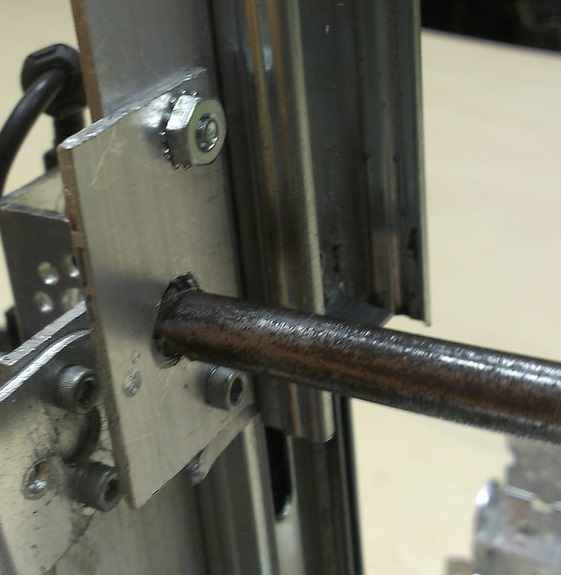
\includegraphics[scale=0.2]{days/24.12.14/images/01}}
			\end{minipage}
			\hfill
			\begin{minipage}[h]{0.29\linewidth}
				\center{
\includegraphics[scale=0.2]{days/24.12.14/images/02}}
			\end{minipage}
			\hfill
			\begin{minipage}[h]{0.2\linewidth}
				\center  
			\end{minipage}
			\caption{Места крепления оси}
		\end{figure}
		
		\item Поскольку у нас не было на занятии паяльника, нам пришлось купить дешевый паяльник.
		
        \item После того, как часть проводов была залужена, паяльник вышел из строя. Было решено, принести на следующее занятие хороший паяльник из дома.
        
        \item Сегодня снова сломалась одна из мебельных реек: нижняя с левой стороны, длиной 30 см. Ее необходимо заменить к тому моменту, как мы закончим запланированную работу над нижней частью робота и перейдем к подъемнику.

	\end{enumerate}
	
	\item Итоги собрания:
	\begin{enumerate}
		
		\item Ось укреплена.
		
		\item Часть проводов залужена.
		
		\item Сломалась одна из реек подъемника.
		
	\end{enumerate}
	
	\item Задачи для последующих собраний:
	\begin{enumerate}
		
		\item Заменить сломанную рейку.
		
		\item Закончить облуживание проводов.
			
	\end{enumerate}
\end{enumerate}
\fillpage
